%; whizzy chapter -dvi
% -initex iniptex -latex platex -format platex -bibtex jbibtex -fmt fmt
% 以上 whizzytex を使用する場合の設定。

%     Tokyo Debian Meeting resources
%     Copyright (C) 2012 Junichi Uekawa
%     Copyright (C) 2011, 2015 Nobuhiro Iwamatsu

%     This program is free software; you can redistribute it and/or modify
%     it under the terms of the GNU General Public License as published by
%     the Free Software Foundation; either version 2 of the License, or
%     (at your option) any later version.

%     This program is distributed in the hope that it will be useful,
%     but WITHOUT ANY WARRANTY; without even the implied warranty of
%     MERCHANTABILITY or FITNESS FOR A PARTICULAR PURPOSE.  See the
%     GNU General Public License for more details.

%     You should have received a copy of the GNU General Public License
%     along with this program; if not, write to the Free Software
%     Foundation, Inc., 51 Franklin St, Fifth Floor, Boston, MA  02110-1301 USA

%  preview (shell-command (concat "evince " (replace-regexp-in-string "tex$" "pdf"(buffer-file-name)) "&"))

%%ここからヘッダ開始。

\documentclass[mingoth,a4paper]{jsarticle}
\usepackage{monthlyreport}
% 日付を定義する、毎月変わります。
\newcommand{\debmtgyear}{2019}
\newcommand{\debmtgmonth}{6}
\newcommand{\debmtgdate}{15}
% started from zero:
% (let ((year 2013) (month 7)) (+ (* (- year 2005) 12) month -1))
\newcommand{\debmtgnumber}{175}

% Needed to import pandoc-generated LaTeX documents.
% See https://stackoverflow.com/questions/40438037/tightlist-error-using-pandoc-with-markdown
\providecommand{\tightlist}{%
  \setlength{\itemsep}{0pt}\setlength{\parskip}{0pt}}

\begin{document}

\begin{titlepage}
\thispagestyle{empty}
% タイトルページ:編集必要な部分は最初のマクロに飛ばすこと

\vspace*{-2cm}
第\debmtgnumber{}回 東京エリア Debian 勉強会資料\\
\hspace*{-2cm}

\includegraphics{image2012-natsu/dotdeb.pdf}\\
\hfill{}\debmtgyear{}年\debmtgmonth{}月\debmtgdate{}日

% ここはアップデートすること
% 全角文字にしないとフォントのサイズが合わないので注意
\rotatebox{10}{\fontsize{30}{30} {\gt OSC北海道報告&コミュニティ検討}}\\

\vspace*{-2cm}
\hfill{}
\includegraphics[height=6cm]{image200502/openlogo-nd.eps}
\end{titlepage}

\newpage

\begin{minipage}[b]{0.2\hsize}
 \definecolor{titleback}{gray}{0.9}
 \colorbox{titleback}{\rotatebox{90}{\fontsize{80}{80} {\gt デビアン勉強会} }}
\end{minipage}
\begin{minipage}[b]{0.8\hsize}
\hrule
\vspace{2mm}
\hrule
\begin{multicols}{2}
\tableofcontents
\end{multicols}
\vspace{2mm}
\hrule
\end{minipage}

\dancersection{最近のDebian関連のミーティング報告}{杉本 典充}

\subsection{第174回東京エリアDebian勉強会}

2019年5月18日(土)に第174回東京エリアDebian勉強会を開催しました。会場は東銀座にある朝日ネットさんをお借りして行いました。参加者は5名でした。

セミナー発表は、吉野さんの「/usr Mergeについて」でした。/usr Mergeとは何か、Debianにおける/usr Mergeの進捗度合い、Debian 技術委員会における議論の内容を説明しました。

その後Hack Timeを行い、各自が用意した課題に取り組みました。


\dancersection{事前課題}{dictoss}

今回の事前課題は以下です。

\begin{enumerate}
\item Hack Timeは何をしますか (How will you work on Hack Time ?)
\end{enumerate}

%この課題に対して提出いただいた内容は以下です。

\begin{multicols}{2}
{\small
\begin{prework}{ yy\_y\_ja\_jp }
  \begin{enumerate}
  \item ($B2sEz$J$7(B)
  \end{enumerate}
\end{prework}

\begin{prework}{ tinypiece }
  \begin{enumerate}
  \item Debian(rasbian) $B$K(B kubenetes $B%/%i%9%?!<$rAH$s$G$_$^$9(B
  \end{enumerate}
\end{prework}

\begin{prework}{ koedoyoshida }
  \begin{enumerate}
  \item ($B2sEz$J$7(B)
  \end{enumerate}
\end{prework}

\begin{prework}{ dictoss }
  \begin{enumerate}
  \item GCP$B$NI8=`(BDebian$B$NCf?H$N@_Dj$,$I$&$J$C$F$$$k$+D4$Y$k(B
  \end{enumerate}
\end{prework}

}
\end{multicols}

%\dancersection{Debian Trivia Quiz}{username}
%
%Debianの昨今の話題についてのQuizです。
%
%今回の出題範囲は\url{debian-devel-announce@lists.debian.org} や \url{debian-news@lists.debian.org}などに投稿された内容からです。
%
%\begin{multicols}{2}
%%; whizzy-master ../debianmeetingresume201211.tex
% $B0J>e$N@_Dj$r$7$F$$$k$?$a!"$3$N%U%!%$%k$G(B M-x whizzytex $B$9$k$H!"(Bwhizzytex$B$,MxMQ$G$-$^$9!#(B
%

\santaku
{DebConf13 $B$N3+:ECO$H3+:EF|$O!)(B}
{$BF|K\!"El5~ET(B 6$B7n(B20$BF|(B}
{$B%K%+%i%0%"(B $B%^%J%0%"(B 7$B7n(B8-14$BF|(B}
{$B%9%$%9!"%t%)!<%^%k%-%e(B 8$B7n(B11-18$BF|(B}
{3}
{$B%K%+%i%0%"$O(BDebConf12$B$N3+:ECO$G$9!#(B
DebConf13$B$O%9%$%9$N%-%c%s%WCO$G3+:E$G$9!#(B
6/20$B$O3'$5$sM=Dj$r6u$1$F$*$-$^$7$g$&!#(B}

\santaku
{$B@$3&$N(BWeb$B%5!<%P$G:G$b?M5$$N$"$k(BLinux $B%G%#%9%H%j%S%e!<%7%g%s(B(W3Techs$BD4$Y(B)$B$O!)(B}
{CentOS}
{Debian}
{Ubuntu}
{B}
{\url{http://w3techs.com/technologies/history_details/os-linux}$B$K7k2L$N%0%i%U$,$"$j$^$9!#(B
$B8=:_(B Linux $B$r;HMQ$7$F$$$k(B web $B%5!<%P$N(B 32.9\% $B$,(B Debian $B$rMxMQ$7$F$*$j!"$=$N3d9g$O8=:_$bA}2C$rB3$1$F$$$k$=$&$G$9!#(B}

\santaku
{Debian $B%+!<%M%k%A!<%`$N%a%s%P!<$G$"$j!"(Bkernel.org $B$N(B 3.2.y $B0BDjHG7ONs$N%a%s%F%J$G$b$"$k(B Ben Hutchings $B$5$s$,<!4|(B Debian $B0BDjHG$H0l=o$K=P2Y$5$l$k(B Linux $B%+!<%M%k$K(B (3.2 $B7ONs$N(B mainline $B$K$OL5$$(B) $BDI2C5!G=$,Ek:\$5$l$kM=Dj$G$"$k$H=R$Y$F$$$^$9!#(B
$BB?$/$NDI2CE@$NCf$K4^$^$l$J$$$b$N$O2?!)(B}
{PREEMPT\_RT}
{Hyper-V guest drivers$B$N6/2=(B}
{ARM64/AArch64$B%"!<%-%F%/%A%c%5%]!<%H(B}
{C}
{Hyper-V guest drivers$B$O(Bmainline kernel$B$G(B3.2$B$K$b4^$^$l$F$$$^$9$,!"$h$j2~A1$5$l$?(B3.4$B$+$i$N=$@5$,F3F~$5$l$^$9!#(B
PREEMPT\_RT$B$O%O!<%I%j%"%k%?%$%`$r<B8=$9$k$?$a$N(BPatch$B!"(B
linux-image-rt-amd64 , linux-image-rt-686-pae $B$N(Bmetapackage$B$G;HMQ$G$-$^$9!#(B
$B?7$7$$(BARM 64$B%S%C%H%"!<%-%F%/%A%c%5%]!<%H$O(Bmainline kernel 3.7$B$+$i(B}

\santaku
{Wookey$B$5$s$,%"%J%&%s%9$7$?(Balpha$BHG$N(BDebian port arm64 image$B$O!)(B}
{Debian/Ubuntu port image}
{Debian/KFreeBSD port image}
{Debian/GnuHurd port image}
{A}
{self-bootstrapp(non x86)$BBP1~$H$N$3$H$G$9!#(B\url{http://wiki.debian.org/Arm64Port}$B$G%9%F!<%?%9$,3NG'$G$-$^$9!#(B}

\santaku
{700,000$BHVL\$N%P%0$,Js9p$5$l$?F|$rEv$F$k(B700000thBugContest$B$N7k2L$,=P$^$7$?!#$=$NM=A[F|$HJs9pF|$O!)(B}
{2012/12/12$B$rM=A[$7$?(BDavidPrevot}
{$BM=A[F|(B:2013/02/04$B!"Js9pF|(B:2013/02/14}
{$BM=A[F|(B:2013/02/07$B!"Js9pF|(B:2013/02/14}
{$BM=A[F|(B:2013/02/14$B!"Js9pF|(B:2013/02/07}
{C}
{$B:G$b6a$$(B2013/02/14$B$rM=A[$7$?(BChristian Perrier$B$5$s$,Ev$F$^$7$?!#7k2L$O(B\url{http://wiki.debian.org/700000thBugContest}$B$G8x3+$5$l$F$$$^$9!#(B
$B$^$?!"(B800,000/1,000,000$BHVL\$N%P%0$,Js9p$5$l$kF|$rEv$F$k%3%s%F%9%H(B\url{http://wiki.debian.org/800000thBugContest}$B$b3+:E$5$l$F$$$^$9!#(B}

\santaku
{master.debian.org$B$,?7$7$$5!3#$K0\9T$5$l$^$7$?!#$3$l$O2?$N%5!<%P$G$7$g$&$+(B $B!)(B}
{@debian.org$B$N%a!<%k%5!<%P(B}
{$B%Q%C%1!<%8$N%^%9%?!<%5!<%P(B}
{$B%Q%C%1!<%8$N%9%]%s%5!<(B(mentor)$B$rC5$9%5!<%P(B}
{A}
{$B8E$$%5!<%P$O%G%#%9%/>c32Ey$,$"$C$?$N$G!"<wL?$HH=CG$5$l!"%G!<%?$,B;<:$9$kA0$K?7$7$$%5!<%P$K0\9T$5$l$^$7$?!#(Bftp-master.debian.org$B$O(BDebian$B$N(B official package $B%j%]%8%H%j$G$9!#%Q%C%1!<%8$N%9%]%s%5!<(B(mentor)$B$rC5$9$N$O(Bmentors.debian.net$B!#(B }

\santaku
{pbuilder$B$K(Bclang support$B$,DI2C$5$l$^$7$?!#C/$,=q$$$?%Q%C%A$G$7$g$&$+!)(B}
{Sylvestre Ledru}
{Junichi Uekawa}
{Hideki Yamane}
{C}
{Debian$B$N(BClang$B%5%]!<%H$OCe!9$H?J$s$G$$$^$9!#(B}

\santaku
{DPN - 2013$BG/(B3$B7n(B4$BF|9f$K<h$j>e$2$i$l$?F|K\$N%$%Y%s%H$O(B}
{Open Source Conference 2013 Tokyo/Spring}
{Open Source Conference 2013 Hamamatu}
{Open Source Conference 2013 Tokushima}
{A}
{\url{http://henrich-on-debian.blogspot.jp/2013/02/open-source-conference-2013-tokyospring.html} $B>\:Y$O8e$[$I!#(B}


%\end{multicols}


% % (query-replace-regexp "<.*?>" "")
% % (query-replace-regexp "^[    ]\+" "")

%-------------------------------------------------------------------------------
\dancersection{OSC 2019 Hokkaidoのイベント参加報告と今後の課題整理}{dictoss}
%-------------------------------------------------------------------------------


\subsection{本レポートについて}

北海道でDebian / Ubuntu ユーザーミートアップ in 札幌 2019.05、OSC 2019 Hokkaido のイベントを開催しました。

本レポートは、北海道におけるイベント開催のレポートになります。


\subsection{Debian / Ubuntu ユーザーミートアップ in 札幌 2019.05}


\subsubsection{イベント概要}

\begin{itemize}
\item イベント名
  \begin{itemize}
  \item Debian / Ubuntu ユーザーミートアップ in 札幌 2019.05
  \end{itemize}
\end{itemize}

\begin{itemize}
\item イベントのwebサイト
  \begin{itemize}
  \item \url{https://debianjp.connpass.com/event/126637/}
  \end{itemize}
\end{itemize}

\begin{itemize}
\item 日時
  \begin{itemize}
  \item 2019-05-31(金) 19:00-21:00
  \end{itemize}
\end{itemize}

\begin{itemize}
\item 場所
  \begin{itemize}
  \item 株式会社インフィニットループ様 会議室(サッポロファクトリー1条館 3階)
  \end{itemize}
\end{itemize}


\subsubsection{イベントの来場者}

\begin{itemize}
\item 合計 3名
  \begin{itemize}
  \item 開催側
    \begin{itemize}
    \item 杉本さん、吉野さん
    \end{itemize}
  \item 参加者
    \begin{itemize}
    \item 北野大地@JI8GRX さん
      \begin{itemize}
      \item Debian古参ユーザで、北海道Linuxユーザーズクラブ(DoLUC)\footnote{現在、DoLUCは活動を停止中。}のメンバ
      \item 2017年、2018年のミートアップの参加実績あり
      \end{itemize}
    \end{itemize}
  \end{itemize}
\end{itemize}


\subsubsection{セミナー}

\begin{itemize}
\item 予定していたセミナーはキャンセル(参加者と話し合い、キャンセルとした)
\item 北海道のDebianユーザや北海道のコミュニティの現状を共有することにした
\item キャンセルとなったセミナー
  \begin{itemize}
  \item golangの"net/http/fcgi"を使ってREST APIアプリを作る (発表者:dictossさん)
  \item Debian と セキュアブート (発表者:yy\_y\_ja\_jpさん)
  \end{itemize}
\end{itemize}

  
\subsubsection{情報交換した内容、出てきた意見}

\subsubsubsection{北海道のIT勉強会の現状}
  
\begin{itemize}
\item  LOCALがまとめた北海道のおける勉強会一覧の資料
  \begin{itemize}
  \item \url{https://www.local.or.jp/wp-content/uploads/2019/05/Handbook-2019-19052903.pdf}
  \end{itemize}
\item 上記資料の勉強会はどのような勉強会であるか調べた
  \begin{itemize}
  \item イベント系の団体
    \begin{itemize}
    \item オープンソースカンファレンス北海道実行委員会
    \item 一般社団法人LOCAL
      \begin{itemize}
      \item OSC北海道のイベント実務の大部分はLOCALがやっている
      \end{itemize}
    \item ET ロボコン北海道地区実行委員会
      \begin{itemize}
      \item 北海道の高専は高専ロボコン全国大会の強豪校
      \end{itemize}
    \item U-16プログラミングコンテスト
    \end{itemize}
  \item 学生が主な参加者の勉強会や団体
    \begin{itemize}
    \item LOCAL学生部
      \begin{itemize}
      \item 属している学生の学校は北海道各地に散らばっている
      \item 【疑問】どうやって交流や話をしているのか?\footnote{後述のOSC 2019 Hokkaidoで学生に実際にヒアリングを行った。}
      \end{itemize}
    \item FuraIT(富良野)・ゆるい勉強会(旭川)
      \begin{itemize}
      \item 富良野と旭川の高校生・高専生が主な参加者に見える
      \item 参加者の一部のの人は両方のイベントに参加している(生活圏内が近いためと思われる)
      \end{itemize}
    \item 子ども向け
      \begin{itemize}
      \item TEAM IchigoJam ほっかいどう
      \item CoderDojo 札幌 × 札幌東 × 恵庭
      \end{itemize}
    \end{itemize}
  \end{itemize}
\end{itemize}


\subsubsubsection{北海道の工学系の大学や高校}

\begin{itemize}
\item 北海道大学
  \begin{itemize}
  \item OSC北海道で例年参加者を見かける
  \end{itemize}
\item 室蘭工業大学
  \begin{itemize}
  \item OSC北海道で例年参加者を見かける
  \end{itemize}
\item 北見工業大学
\item 公立はこだて未来大学
  \begin{itemize}
  \item OSC北海道で例年参加者を見かける
  \end{itemize}
\item 公立千歳科学技術大学
  \begin{itemize}
  \item OSC北海道で例年参加者を見かける
  \end{itemize}
\item 札幌市内の私大の工学部系
\item 国立高専(旭川、函館、釧路、苫小牧)
  \begin{itemize}
  \item OSC北海道で例年参加者を見かける
  \end{itemize}
\item 富良野緑峰高校
\end{itemize}


\subsubsubsection{企業}

\begin{itemize}
\item アットマークテクノさん
  \begin{itemize}
  \item Armadillo というボードをつくっており、OS は Debian を採用
  \end{itemize}
\end{itemize}


\subsubsubsection{今回のOSC北海道の参加予定セミナーの申し込み数の傾向}

\begin{itemize}
\item Microsoftのセミナーは人気が高い
\item Pythonのセミナーは人気が高い
\item VRネタ、AIネタは人気が高い
\item プログラミング教育系のセッションの人気が高い
\item 勉強会そのものの体験談、カンファレンスの参加体験談に人が集まる
\end{itemize}


\subsubsubsection{どうやって大学や高校、学生と接触していくとよいか}

\begin{itemize}
\item 【悩み】先生や学生に接触できればよいが、どうやって接触すればよいかわからない
\end{itemize}


\subsection{オープンソースカンファレンス 2019 Hokkaido}

\subsubsection{イベント概要}

\begin{itemize}
\item イベント名
  \begin{itemize}
  \item オープンソースカンファレンス 2019 Hokkaido
  \end{itemize}
\end{itemize}

\begin{itemize}
\item イベントのwebサイト
  \begin{itemize}
  \item \url{https://www.ospn.jp/osc2019-do/}
  \end{itemize}
\end{itemize}

\begin{itemize}
\item 日時
  \begin{itemize}
  \item 2019-06-01(土) 10:00-18:00
    \begin{itemize}
    \item DebianJPでは、2日目のコミュニティデイのみ参加
    \item ブース展示、セミナーを開催
    \end{itemize}
  \end{itemize}
\end{itemize}

\begin{itemize}
\item 場所
  \begin{itemize}
  \item 札幌コンベンションセンター(地下鉄東西線 東札幌駅近く)
  \end{itemize}
\end{itemize}


\subsubsection{イベントの来場者}

\begin{itemize}
\item 2日間合計で約 720 名程度(主催者発表値)\footnote{出典:メーリングリスト osc-member [osc:7983] [北海道] アンケート集計結果}\footnote{過去データ一覧\url{https://www.ospn.jp/visitors/}}
  \begin{itemize}
  \item 5/31(金) 約  80 名(ビジネスデイ)
  \item 6/01(土) 約 640 名(コミュニティデイ)
  \item 2日間合計  約 720 名
  \end{itemize}
\end{itemize}

\begin{itemize}
\item 学生の参加者比率が高い
  \begin{itemize}
  \item 高校生、高専生、大学生が参加している
  \item 交流した学生で学校が判明しているところ
    \begin{itemize}
    \item 公立千歳科学技術大学
    \item 公立はこだて未来大学
    \item 室蘭工業大学
    \item 北海道大学
    \item 苫小牧高専
    \item 旭川高専
    \item 旭川工業高校
    \end{itemize}
  \end{itemize}
\end{itemize}


\subsubsection{セミナー}

\begin{itemize}
\item 公開プログラム
  \begin{itemize}
  \item \url{https://www.ospn.jp/osc2019-do/modules/eventrsv/?id=2&noform=1}
  \item 2019/6/1(土) 11:00-11:45
  \end{itemize}
\end{itemize}

\begin{itemize}
\item 発表内容
  \begin{itemize}
  \item タイトル「Debian Updates」
  \item 発表者は杉本さん
  \item スライド資料\footnote{\url{https://tokyodebian-team.pages.debian.net/pdf2019/debianmeetingresume201906-osc2019do-presentation.pdf}}
  \end{itemize}
\end{itemize}

\begin{itemize}
\item 聴講者
  \begin{itemize}
   \item 6名
  \end{itemize}
\end{itemize}


\subsubsection{ブース展示}

\begin{itemize}
\item 2019/6/1(土)のみ展示
  \begin{itemize}
  \item 吉野さん、杉本さんで対応
  \end{itemize}
\end{itemize}

\begin{itemize}
\item 出展内容
  \begin{itemize}
  \item Debian GNU/Linux マシンのデモ展示
  \item Debian管理者ハンドブックの展示
  \item トイストーリーのキャラクターのぬいぐるみ展示
  \item Debian勉強会のチラシ配布
  \item Debian シール配布(スーパーキー/スケルトン)
  \item Debian勉強会の過去のまとめ冊子展示/販売
  \item Debian Tシャツ販売  
  \end{itemize}
\end{itemize}

\begin{figure}[H]
  \begin{center}
    % \url{https://twitter.com/dictoss/status/1134624475486380032}
    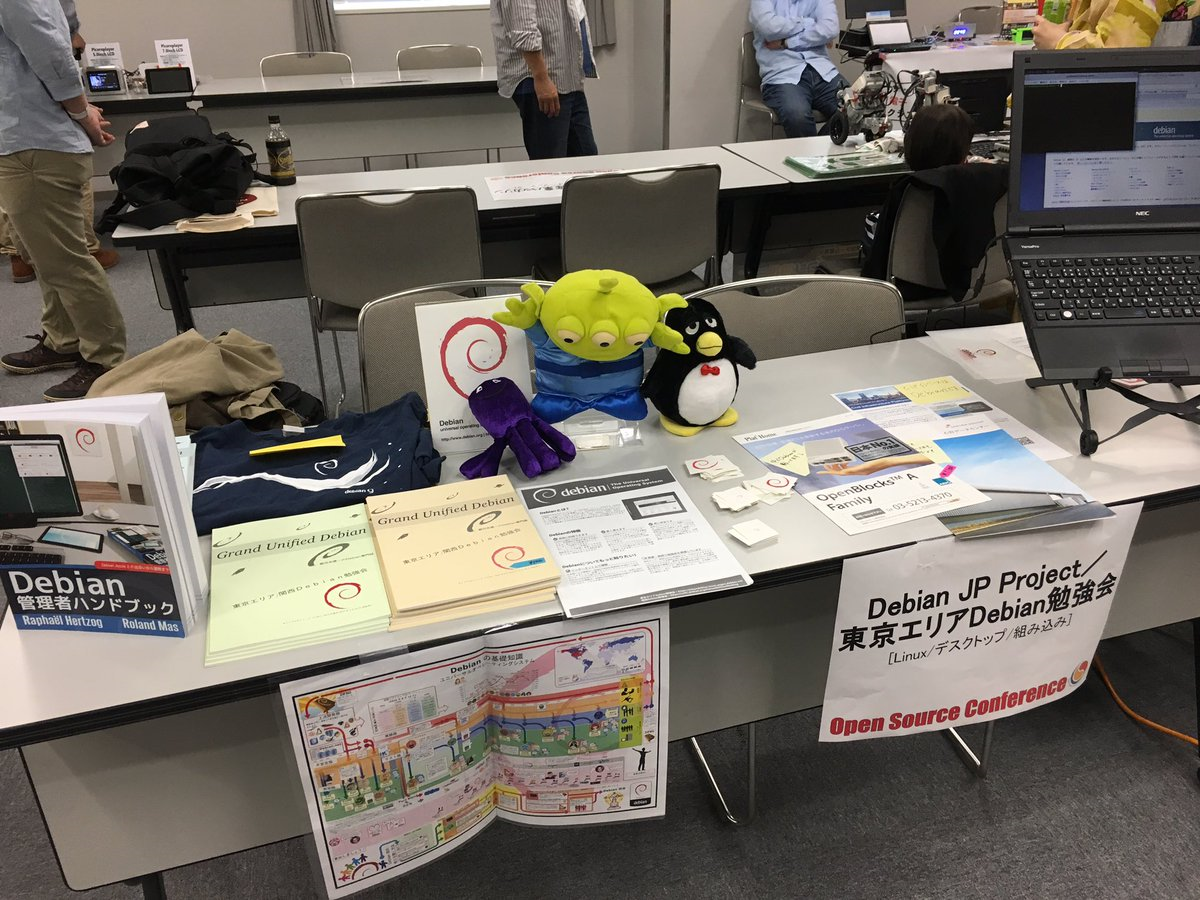
\includegraphics[width=12cm]{image201906/debianjp-booth_osc2019do.png}
    \caption{展示ブースの様子(OSC 2019 Hokkaido)}
    \label{fig:booth-osc2019do}
  \end{center}
\end{figure}

\begin{itemize}
\item ブース来訪者
  \begin{itemize}
  \item 合計 約 61 名
  \item 属性
    \begin{itemize}
    \item 男性・大人     30 名
    \item 女性・大人      5 名
    \item 男性・学生子供 25 名
    \item 女性・学生子供  1 名
    \end{itemize}
  \end{itemize}
\end{itemize}

\begin{itemize}
\item 物販
  \begin{itemize}
  \item 本:あんどきゅめんてっどでびあん\footnote{\url{https://tokyodebian-team.pages.debian.net/undocumenteddebian.html}}
    \begin{itemize}
    \item 3 冊販売
    \end{itemize}
  \item Debian Tシャツ
    \begin{itemize}
    \item 4 着販売
    \end{itemize}
  \end{itemize}
\end{itemize}


\subsubsection{ブース来訪者との情報交換}

\begin{itemize}
\item 利用OSのアンケート
  \begin{itemize}
  \item Ubuntu     10
  \item Debian      7
  \item Raspbian    4
  \item ChromeOS    1
  \item EV3 Debian  1
  \item CentOS      1
  \end{itemize}
\end{itemize}


\subsubsection{イベントの参加者や出展者との交流}

\begin{itemize}
\item LOCAL学生部
  \begin{itemize}
  \item メンバは北海道各地に散らばっている
  \item 主にslackでコミニケーションをとっている
  \item Face to Faceで会うのはOSCとそれ以外に年に1回程度
  \item 「LOCAL Students 情報ボーイズの寄稿ノート」という本を出している\footnote{\url{https://techbookfest.org/event/tbf04/circle/14720002}}\footnote{原稿はtexで書いている模様。\url{https://github.com/hyoiutu/techbookfest_localstudents_2017}}\footnote{2冊目にあたる「LOCAL Students 情報ボーイズの寄稿ノート 2.0」を当日販売していた。}
  \end{itemize}
\end{itemize}

\begin{itemize}
\item 深町先生
  \begin{itemize}
  \item 公立千歳科学技術大学の先生
  \item FMLの開発者
  \end{itemize}
\end{itemize}


\subsection{今後のDebian開発者候補の方への呼びかけ方のディスカッション}

\subsubsection{観点}

\subsubsubsection{会いに行く・会いに来る}
  
\begin{itemize}
\item 東京圏におけるイベントと地方におけるイベントの傾向の違い
\item 高校生・高専生・専門学校生・大学生におけるイベントや勉強会の参加の壁は何か(時間、金銭、距離など)
\item 学生のいる場所へ呼んでもらう方法
\item 先生とどう知り合い、どのような情報交換をしていくとよいか
\end{itemize}

\subsubsubsection{Debian勉強会における情報提供の在り方}

\begin{itemize}
\item 取り上げる話題をどう選んでいくか
  \begin{itemize}
  \item 時事ネタ、流行りネタ、利用事例
  \item インストール
  \item アプリケーション、ミドルウェアの利用
  \item 開発環境
  \item Debianの仕組み解説
  \end{itemize}
\item Debian勉強会の資料をどのようなメディアで提供するとよいか
\item Debian勉強会のセミナーのビデオ配信(ライブまたは録画)の是非
\end{itemize}

\subsubsubsection{インターネットにおける情報提供}

\begin{itemize}
\item メーリングリスト
\item ブログ記事
\item webサイト
\end{itemize}

\subsubsubsection{イベントやセミナーにおける情報提供}

\begin{itemize}
\item セミナーのテーマに取り上げる話題の選定
  \begin{itemize}
  \item OSCでは「Debian Update」という半年間を振り返る話をすることが多い。見直すべきか?
  \end{itemize}
\item 魅力あるブース展示にするための検討
\item イベントの参加者属性を意識する
  \begin{itemize}
  \item OSCは入門者向けのイベントのため、セミナーは入門レベルの難易度に設定している
  \item より高度な知識を求める人はどのようなイベントに集まるか?また、そのイベントにDebian勉強会はどう関わるか?
  \end{itemize}
\end{itemize}


% 冊子にするために、4の倍数にする必要がある。
% そのための調整
%\dancersection{メモ}{}
\mbox{}\newpage

\vspace*{15cm}
\hrule
\vspace{2mm}

\includegraphics[width=2cm]{image200502/openlogo-nd.eps}
\noindent \Large \bf Debian 勉強会資料\\
\noindent \normalfont \debmtgyear{}年\debmtgmonth{}月\debmtgdate{}日 \hspace{5mm}  初版第1刷発行\\
\noindent \normalfont 東京エリア Debian 勉強会 (編集・印刷・発行)\\
\hrule

\end{document}
